% Setup - do not change
\documentclass[11pt]{article}
\usepackage[top=0.9in, left=0.9in, bottom=0.9in, right=0.9in]{geometry} 
\usepackage{parskip}
\usepackage{multicol}
\usepackage[english]{babel}
\usepackage[utf8]{inputenc}
\usepackage{amsmath,amsthm,amssymb,graphicx,pdfpages,lipsum,hyperref}
\usepackage[none]{hyphenat}
\usepackage{csquotes}
\usepackage{float}


\setlength\parindent{0pt}
%%%%%%%%%%%%%%%%%%%%%%%%%%%%%%%%%%%%%%%%%%%%%%%%%%%%%%%%%%%%%%%%%%%
% add other packages here if required

%% Bibliography are specified in this file. You can also choose inline bib style if you want to. But make sure your citation style is consistent (and proper)
% For more details on citation: https://library.unimelb.edu.au/recite
\usepackage[sorting = none]{biblatex}
\addbibresource{references.bib}

%%%%%%%%%%%%%%%%%%%%%%%%%%%%%%%%%%%%%%%%%%%%%%%%%%%%%%%%%%%%%%%%%%% the '%' symbol denotes comments

% Begin document creation
% DELETE THE \lipsum PLACEHOLDERS WHEN YOU BEGIN
\title{\textbf{How Does Viral Infection Affect Taxi Service Reliance?} \\ 
MAST30034 Assignment 1}
\author{
Xavier Travers \\
Student ID: 1178369 \\
%% Replace the link with your github repo
% 1. Remember to escape underscore in the link.
% 2. Remember to include the commit you want to submit in the link
TODO: \href{https://github.com/MAST30034-Applied-Data-Science/mast30034\_p1\_template/tree/fd9f1dd17fdbcb5b119b70c93a22da8210d44fd7}{Github Repository}
}

\begin{document}
\maketitle

\section{Introduction}
% Link to a 30 min tutorial if you require revision: https://www.overleaf.com/learn/latex/Learn_LaTeX_in_30_minutes

Viral infection is on everyone's mind in the past few years due to the COVID-19 pandemic.
With lockdowns and fears of infection, 
it is a natural assumption that many people-facing industries such as ride-hailing have suffered in demand.
To what extent is such an assumption true?

% TODO: redo this intro section its kinda bad
This report aims to contribute to a body of works attempting to quantify the effect that widespread viruses may have on different industries.

Statistical analysis involved in revealing the extent to which case rates of a viral infection correlates with taxi trip rates and passenger counts.

\subsection{Timeline}
Throughout this report, several timelines are used.
\begin{itemize}
    \item \textbf{Timeline 1:} Starting in March 2018 and ending in February 2021.
    This 36-month timeline is primarily used in visualizations.
    \item \textbf{Timeline 2:} Starting in March 2018 and ending in February 2019.
    This 12-month timeline provides a window of time prior to the COVID-19 pandemic.
    It is used when data analysis focuses only on the effects of the Influenza virus 
    (since the effects of COVID-19 are likely confounding).
    \item \textbf{Timeline 3:} Starting in March 2020 and ending in February 2021.
    This 12-month timeline provides a window of time during the COVID-19 pandemic.
    This timeline is used to construct linear models and perform non-visual data analysis.
\end{itemize}
Data from 2022 is not included, as many of the datasets would be incomplete or unchecked.
Data from before 2018 is not included so that Timeline 2 and Timeline 3 are the same duration (12 months), 
and to reduce code runtime when generating visualizations.

\subsection{Datasets}
\begin{itemize}
    \item The New York City Taxi and Limousine Commission (TLC) provides a dataset of taxi service trips which captures information such as type of taxi, travel distance, general pickup/dropoff locations/times and driver-input passenger counts \cite{tlcdataset}. 
In this report, the focus is placed on New York's Yellow street hail taxis. The dataset provides coverage over the whole of Timeline 1.
Also included from the same source is a mapping dataset for the pickup/dropoff location IDs included in the TLC dataset \cite{tlcdataset}.
    \item Influenza case rates are recorded on a weekly basis by the New York Department of Health \cite{fludataset}. 
Case rates in this dataset are dated based on Morbidity and Mortality Weekly Report (MMWR) weeks, which are generated using rules defined by the CDC \cite{mmwr}.
Each entry in this dataset contains an MMWR week, county (within the state of New York), type of Influenza (A, B or unspecified), and case count.
The dataset provides coverage over the whole of Timeline 1.
    \item COVID-19 case rates have been recorded daily by the New York Department of Health and Mental Hygiene \cite{coviddataset}.
This dataset begins on the last day of february, when the first official cases of COVID-19 were recorded in New York City. 
Each entry in this data set contains a date and several of the daily COVID-19 rates by borough (e.g. count of hospitalizations on the day in the Bronx).
Of specific interest is the daily case count per borough.
    \item Since data is aggregated by borough, the population of each borough needs to be accounted for.
    For this purpose, the United States Census Bureau's yearly county population totals data is used \cite{populations2019, populations2020}.
    This report specifically relies on the population estimates for the counties of New York State.
    \item To provide a homogeneous time metric for aggregation, a dataset is generated which defined the MMWR weeks of the data within the selected timeline.
    The MMWR weeks are generated according to the CDC's defined business rules \cite{mmwr}.
    \item For geospatial visualizations, 
    the City of New York's Department of City Planning provides a dataset containing borough outlines \cite{boroughdataset}.
    This contains the geometry of each borough as well as their names.
\end{itemize}


% \LaTeX{} Have many caveats, you should search stack overflow for latex tips whenever you feel something looks bad, for instance:
% When `` quoting '', should be used instead of ". For example, ``test'' vs "test".

% % use \textbf{} for bold text and \textit{} for italic. 
% % \texttt{} creates code blocks akin to `code ticks` in markdown
% \textbf{Please refer to the spec, the word count and page count is strict.} Feel free to change the section headings (and we recommend you do).

% Always remember to cite materials that does not belong to you. For instance, you should cite the sensor datasets \cite{2022sensorreading, 2022sensorlocation}.
% % Example here used biblatex to manage citations: https://www.overleaf.com/learn/latex/Bibliography_management_with_biblatex , You are free to choose your own way for managing references if biblatex seems too hard.

% \lipsum[7]

% You can have \section{}, \subsection{}, and \subsubsection{}
\section{Method}

\subsection{Preprocessing}

The datasets require several preprocessing steps to generate aggregate data for proper analysis.
The flu dataset contains detail only on a weekly basis, 
while the other datasets contain daily data. 
Thus, the most granular time unit by which the data can be analysed is the MMWR week.
While data per day allows for more data-points in analysis,
Timelines 2 and 3 that ensure around 52 aggregated points of data are available for analysis per per borough.

\subsubsection{Cleaning}

There are several processes used to remove outliers and unwanted data.
Noted are the steps taken to ensure that aggregation by borough and MMWR week is achievable with the TLC, COVID-19 and Influenza datasets.
No imputation is necessary, since the scope of the timelines is very wide (approximately 208 million trips' worth), 
and after removing noise (in the methods described below) from the data, there are still approximately 100 million trips.
Neither the COVID-19 nor the Influenza datasets require imputation, 
since these are maintained to the standards of important medical datasets.

\textbf{Borough vs. County:} Each of the 5 boroughs of New York City correspond to a county recognized by New York State, defined in Table~\ref{tbl:btc} \cite{countytoborough}.
Some datasets contain counties, while others define statistics per borough.

\begin{table}[H]
        \begin{center}
            \begin{tabular}{|l||l|l|l|l|l|} 
            \hline
            Borough Name    & Bronx & Brooklyn  & Manhattan & Queens    & Staten Island \\
            \hline
            County Name     & Bronx & Kings     & New York  & Queens    & Richmond \\
            \hline
            \end{tabular}
            \caption{Mapping Borough Names to County Names in New York City}
            \label{tbl:btc}
        \end{center}
    \end{table}

\textbf{Population Dataset:}
Only data for New York City counties within the years of Timeline 1 is kept.

\textbf{TLC Dataset:}
\begin{multicols}{2}
    \begin{enumerate}
        \item Derive trip duration (in hours) and trip speed (in MPH) columns. 
        Filter out illegal (and likely incorrect) trip entries with a speed greater than 65 MPH, 
        as per New York State law \cite{laws}.
        \item Discard all columns except the pickup time, passenger count, trip distance, pickup location ID, and dropoff location ID.
        \item Discard rows with null values in the above columns or where there is negative distance.
        \item Derive the MMWR week associated to each trip entry, as well as the year and month that the majority of the week participates in.
        Discard all rows where the MMWR week is not within Timeline 1.
        \item For each entry, find the associated pickup borough and dropoff borough. 
        Discard all rows where either of the location IDs are not within the 5 boroughs.
    \end{enumerate}
\end{multicols}

\textbf{COVID-19 Dataset:}
% \begin{multicols}{2}
    \begin{enumerate}
        \item Extract the case count per day per borough. Discard rows with negative case counts.
        \item Derive the MMWR week associated to each day entry, as well as the year and month that the majority of the week participates in.
        Discard all rows where the MMWR week is not within Timeline 1.
    \end{enumerate}
% \end{multicols}

\textbf{Influenza Dataset:}
% \begin{multicols}{2}
    \begin{enumerate}
        \item Discard rows with negative case counts.
        \item Convert counties to their associated borough names for homogeneity of data.
        \item Discard all rows where the MMWR week is not within Timeline 1.
    \end{enumerate}
% \end{multicols}

\subsubsection{Aggregation}

\textbf{TLC Dataset:}

From this dataset, two aggregated datasets are generated.
One aggregated by MMWR week and pickup borough, and the other aggregates by MMWR week and dropoff borough.
This allows for analysis by destination, or starting point of taxi trips.
The aggregated sets are then joined by MMWR year and borough to their corresponding population estimated.
For each of the groupings described above, 
the average trip distance and passenger count is calculated, 
as well as the total number of trips, and the number of trips per capita (derived using the borough's population estimate).

\textbf{COVID-19 Dataset:}

Similarly to the above, the dataset is grouped by MMWR week information and borough.
This grouping is joined by MMWR year and borough with the corresponding population estimates.
For each grouping, the total number of cases and total per capita are calculated.

\textbf{Flu Dataset:}

Similarly to the above, the dataset is grouped by MMWR week information and borough.
This grouping is joined by MMWR year and borough with the corresponding population estimates.
For each grouping, the case total per capita is calculated (the case total per MMWR week per borough is already included).

\subsection{Analysis and Modelling}

\subsubsection{Preliminary Analysis}

It appears that there very clearly is a dip in passengers, 
trip rates and trip distances following the start of the COVID-19 pandemic.

\begin{figure}[h]
    % change the scale multiplier to make the figures smaller or larger
    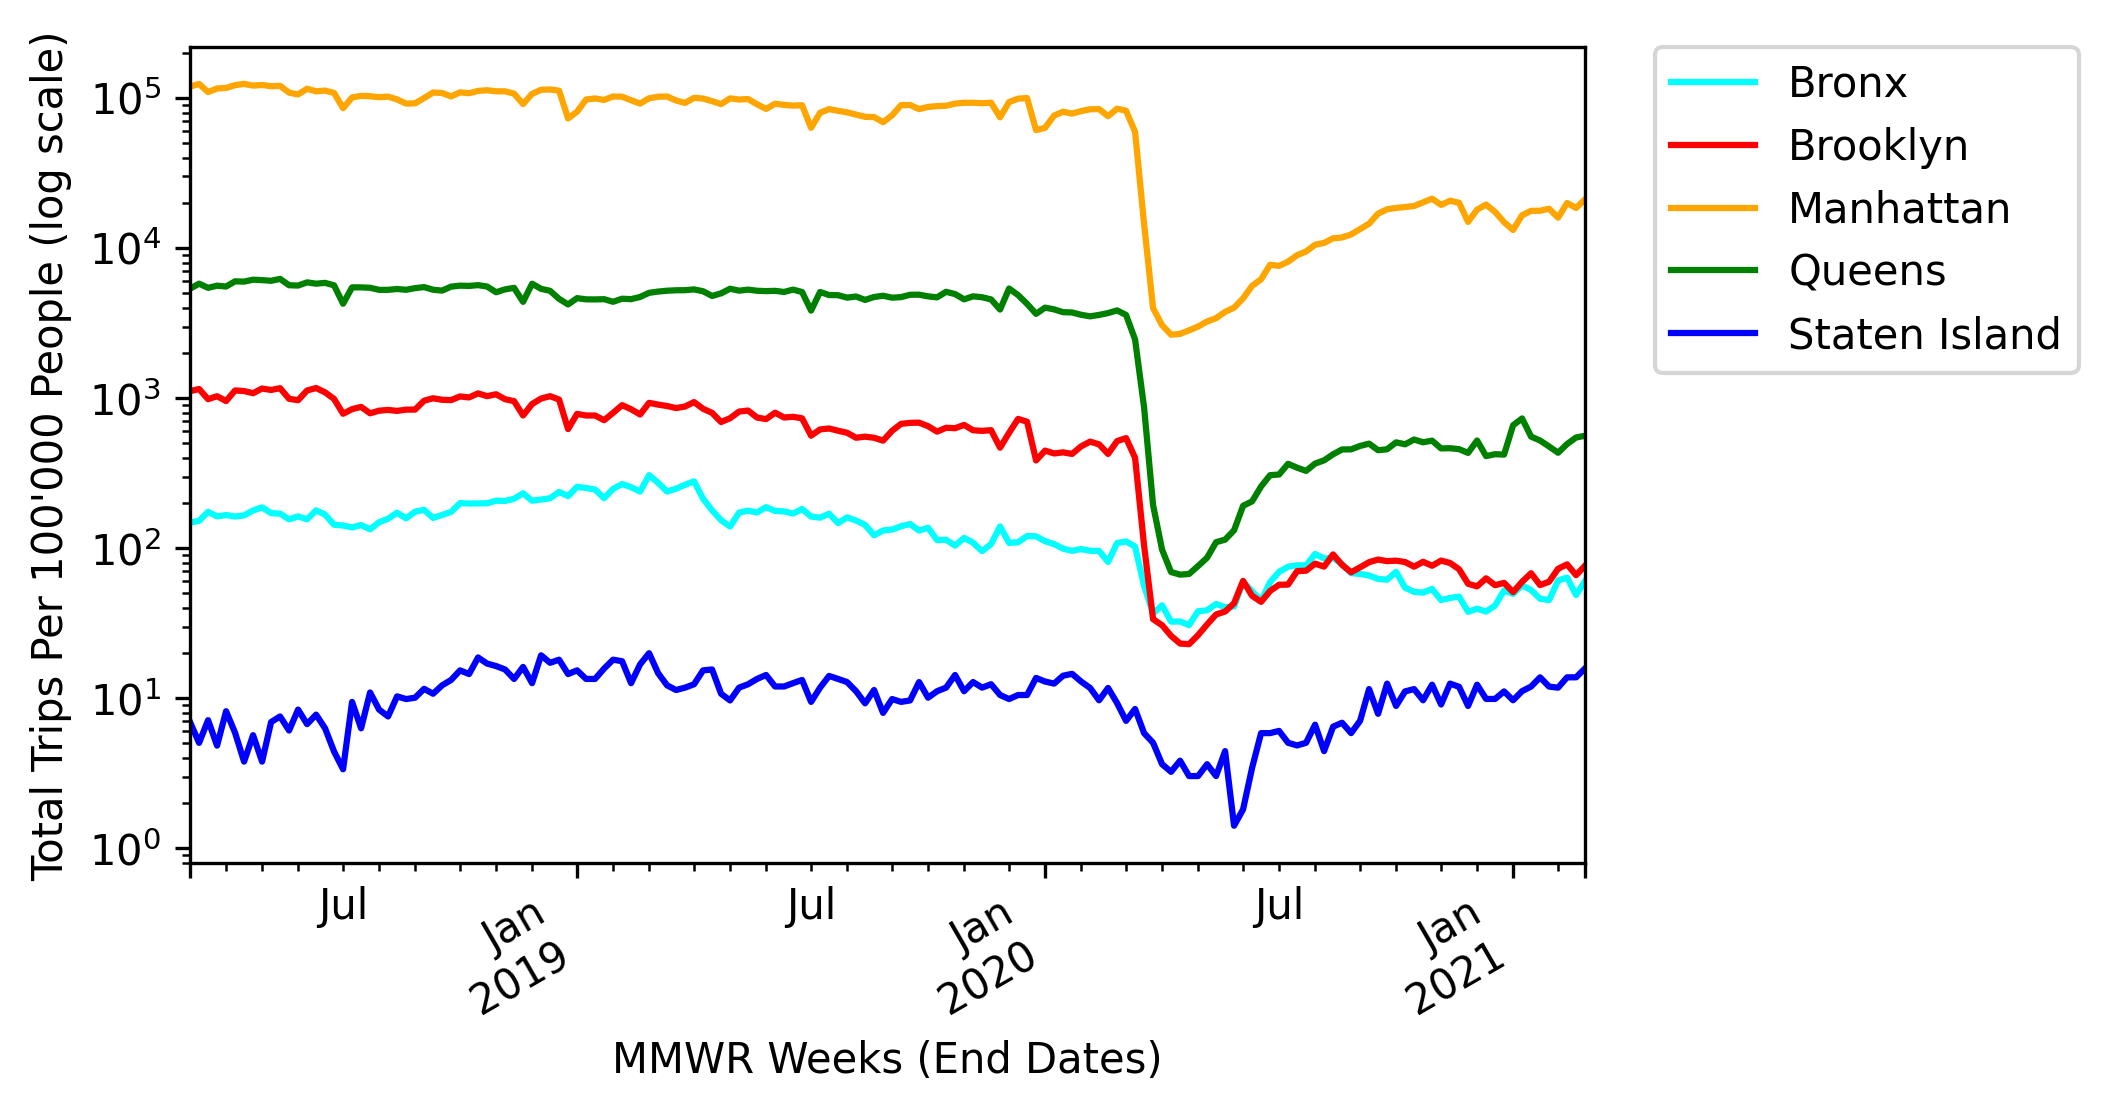
\includegraphics[width=0.45\textwidth]{../plots/time-series-Total Trips Per 100'000 People (log scale)-vs-MMWR Weeks (End Dates)-by-pu_borough.png}
    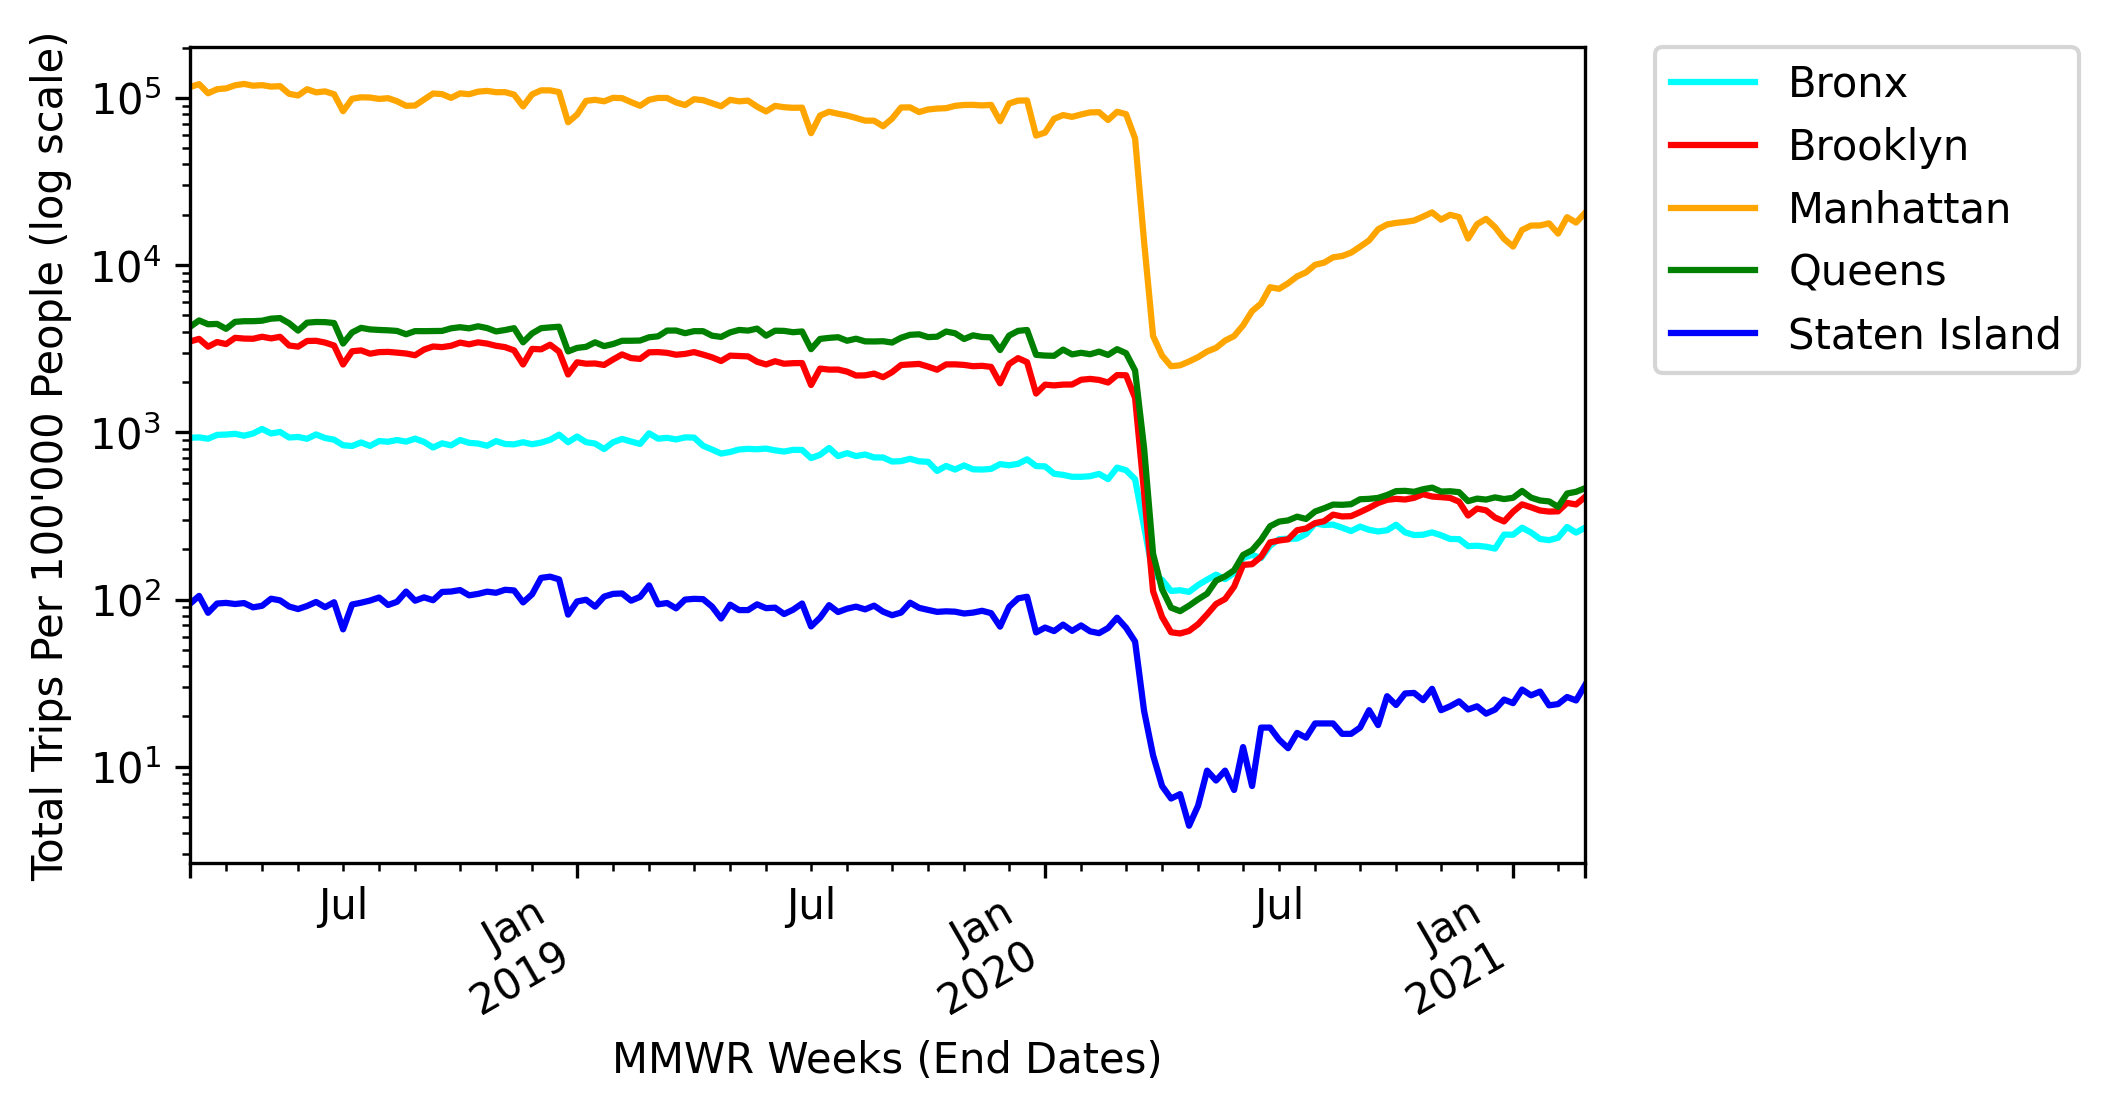
\includegraphics[width=0.45\textwidth]{../plots/time-series-Total Trips Per 100'000 People (log scale)-vs-MMWR Weeks (End Dates)-by-do_borough.png}
    % this ensures your figures are centered where possible
    \centering
    \caption{How trip rates per 100k people per pickup (left) and dropoff (right) borough vary over time.} % refer to this image as (Figure 1)
\end{figure}

% \begin{enumerate} 
%     \item Example for enumerated points
%     % use \item to create more points
% \end{enumerate}

% \begin{itemize} 
%     \item Example for dot points
%     \item[*] You can change dot points to any symbols by putting [SYMBOL].
%     \item[$\times$] Here's a fun example.
% \end{itemize} 
% \lipsum[4-5]
% Example code for figures:
% % the [h] ensures your figure is inline at the location and not displayed on some other page
% \begin{figure}[h]
%     % change the scale multiplier to make the figures smaller or larger
%     \includegraphics[width=0.35\textwidth]{example-image-a}
%     % this ensures your figures are centered where possible
%     \centering
%     \caption{Some caption} % refer to this image as (Figure 1)
% \end{figure}
% \lipsum[1-2]

% Example of a maths equation:
% \begin{equation}
%     Y = X\beta + \epsilon
% \end{equation}

% Example of an aligned equation (\& denotes the symbol to align):
% \begin{align*}
%     E[\mathbf{y}] &= X\beta + E[0] \\
%                   &= X\beta
% \end{align*}

% Example of an in-line equation $\epsilon \sim N(0, 1)$ \\

\subsection{Geospatial Visualisation}

\section{Recommendations}
% \lipsum[10]

\section{Conclusions}
% \lipsum[14-15]


\clearpage

% BEGIN REFERENCES SECTION
\printbibliography

\end{document}